\title{CS 513 Assignment 6}
\author{Ruochen Lin}
\documentclass[11pt]{article}
\usepackage{amsmath,amsfonts,amssymb,amsthm}
\usepackage{mathtools}
\usepackage{commath}
\usepackage{setspace}
% \usepackage{algorithm,algorithmic}
\usepackage{diagbox}
\usepackage{multirow}
\begin{document}
\maketitle
\section{}
If we use the \texttt{rand} function in \texttt{Matlab} to generate a $100\times100$ random matrix, which we denote with $A$, then the typical distribution of the absolute values of its spectrum is shown in Figure. After multiple experiments, we see that there is one eigenvalue that `dominates' over all other eigenvalues in modulus, and it is located around 50. Apart from this outlier, the other eigenvalues are of realatively comparable sizes.\\[0.3cm]

\begin{center}
\begin{figure}[h]
\centering
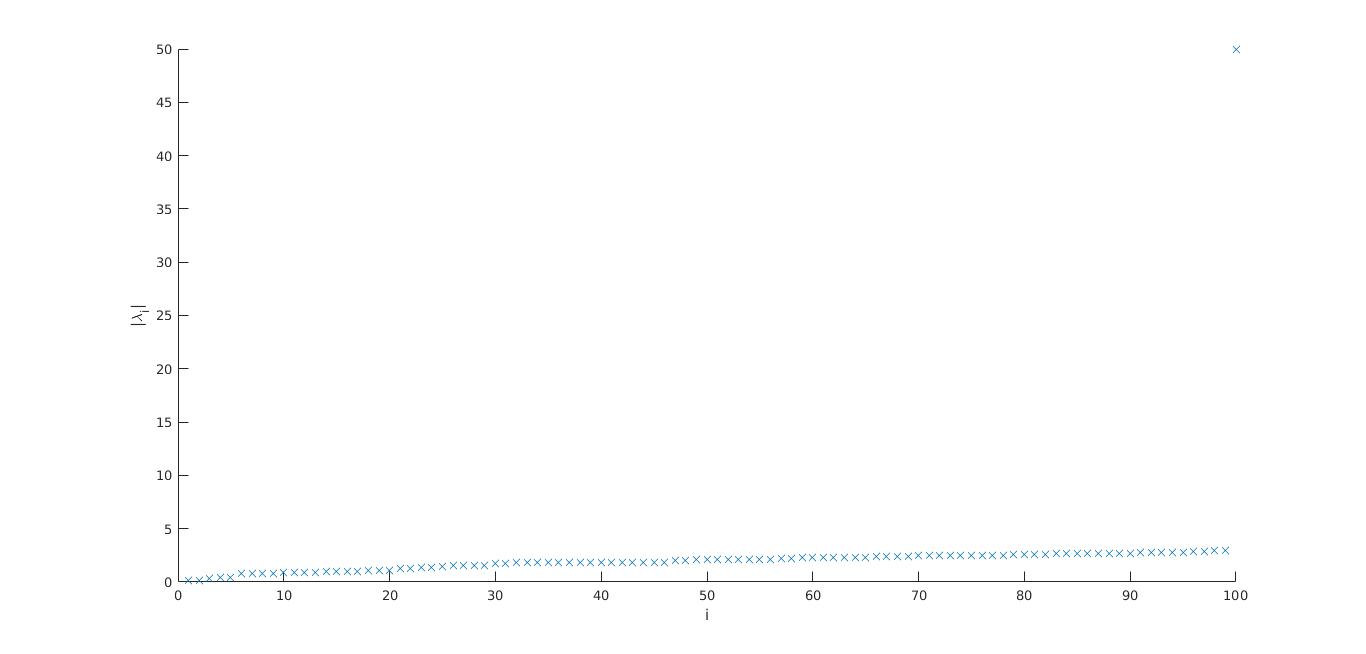
\includegraphics[width=14cm]{matlab/prob1a_uniform.jpg}
\caption{Distribution of $\abs{\lambda_i}$ of a random $100\times100$ matrix generated by \texttt{rand} function.}
\end{figure}
\end{center}

Figure 2 shows the distribution of the spectrum of $A$ and its Arnoldi approximations with $n=1,2,3$ on the complex plane. We see that all of the eigenvalues of $A$ has positive real parts, and the complex eigenvalues of $A$ appear in $\sigma(A)$ with their complex conjugates. This is an expected property for a real matrix. In addition, the convergence of eigenvalues approximated by the Arnoldi method towards the largest eigenvalue is much faster than those to other smaller eigenvalues: even at $n$ values as small as $2$ or $3$, the Arnoldi approximation of the eigenvalue is almost identical to the real value of $\lambda_{\max}$. For the other eigenvalues, however, we do not see any convergence at such small $n$s.
\begin{center}
\begin{figure}[h]
\centering
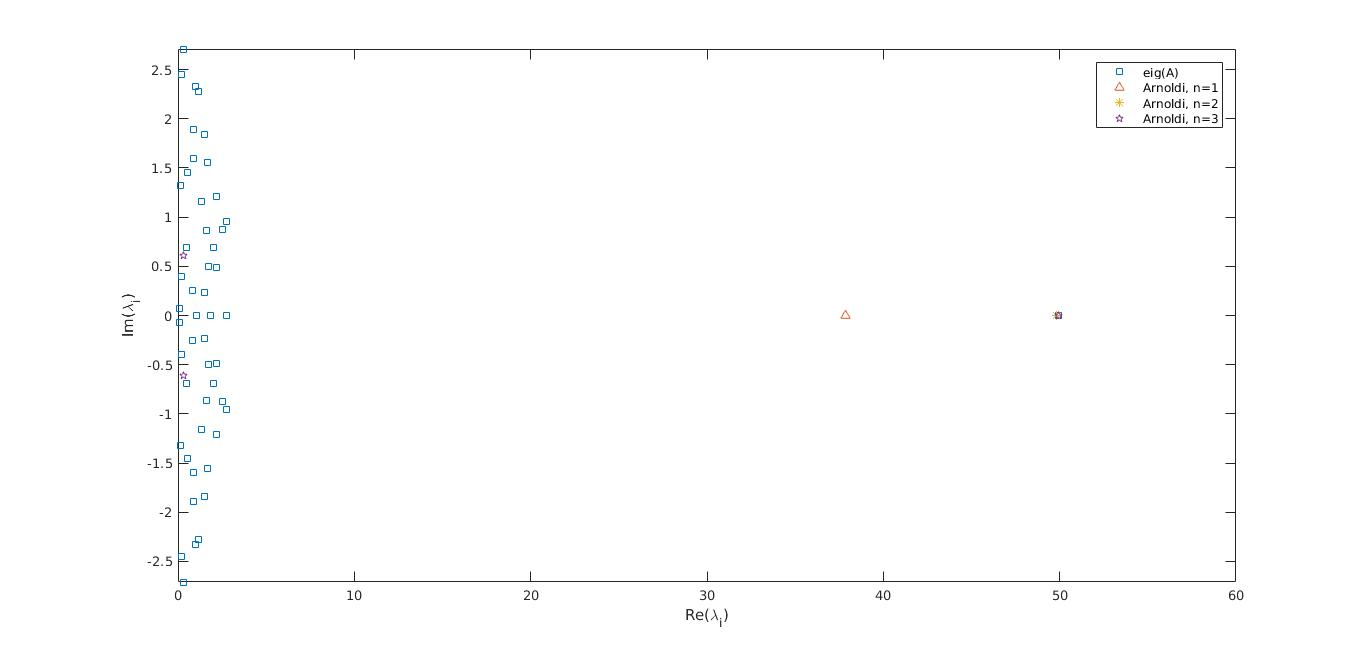
\includegraphics[width=15cm]{matlab/prob1b_uniform.jpg}
\caption{Distribution of $\sigma(A)$ and its Arnoldi approximation at $n=1,2,3$, with $A$ being a random $100\times100$ matrix generated by \texttt{rand} function.}
\end{figure}
\end{center}
The observation from Figure 1 can be explained by the Perron-Frobenius Theorem: when we have a real square matrix with only possitive entries, there will be one real eigenvalue that has its modulus strictly larger than all other eigenvalues. The observation from Figure 2 is explained by the known fact that the Arnoldi iterations give geometric convergence towards the `outlier' eigenvalue in the spectrum of a matrix, and the convergence to other eigenvalues is much slower.
\pagebreak
\section{}
From Table 1 we can see that, if $\epsilon$ is small, GMRES could converge to the correct solution faster. This matches our analysis in class, because in the limit of $\epsilon\to0$, we would expect GMRES to find the solution in 3 steps. Actually, for $\epsilon=10^{-10}$, we do see this type of fast convergence. Another obsevation is that, in general, as $n$ increases, the error becomes smaller. This is the result of an expanding Krylov subspace. However, in the cases of $\epsilon=10^{-4}$ and $10^{-10}$, error increased a bit from the order of $10^{-13}$ to $10^{-12}$ from $n=10$ to $n=90$. This might be the result of error accumulation in numerical computations.
\begin{center}
\begin{table}
\caption{Errors generated in GMRES with different $\epsilon$s and $n$s for a $100\times100$ random matrix with eigenvalues centered around 4, 5, and 10 with radius $\epsilon$.}
\centering
\begin{tabular}[h]{| c |  c c c c |} 
\hline
 & \multicolumn{4}{c|}{$n$} \\
 $-\log_{10}\epsilon$  & 5 & 10 & 20 & 90 \\[0.3ex] \hline
   1  & -3.62 & -9.09 & -12.22 & -12.57 \\
  4  & -6.55 & -13.14 & -12.52 & -12.50 \\
  7  & -8.44 & -12.37 & -12.37 & -12.37 \\
 10  & -12.75 & -13.28 & -13.30 & -12.62 \\\hline
\end{tabular}
\end{table}
\end{center}


\end{document}

